The following section presents the runtime view diagrams for each use case outlined in the RASD v1 document accompanying this report. It covers 17 use cases and illustrates the interactions between the system's components. It is important to note that the API interface artifact has been excluded from the diagrams to avoid unnecessary clutter, as its inclusion offers little to no benefit to the communication process between components. For the sake of simplicity, this section assumes that the API is integrated as part of the AWS Server component.
\newpage
\begin{enumerate}[label={[UC\arabic*]}]
    \item Student and University User Registration
    \begin{figure}[h]
        \centering
        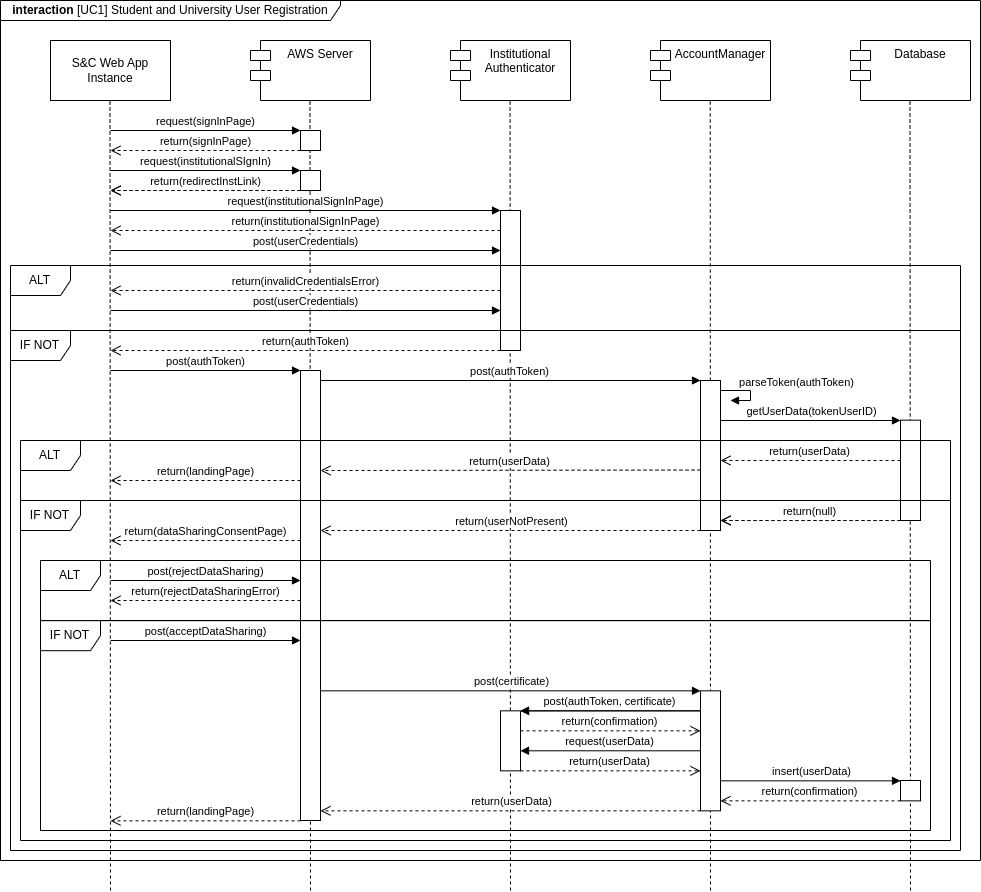
\includegraphics[width=1\linewidth]{DD-Latex//assets//Runtime View Diagrams/UC1.jpg}
        \caption{UC1 - Runtime View Diagram}
        \label{fig:UC1}
    \end{figure}
    
    The diagram in Figure 5 illustrates the interactions between system components during the Student and University user registration process. As noted, the system supports the use of an external authenticator (such as Microsoft 365), which provides the data required to set up a user's profile. The diagram shows the data transfer and storage in the platform's database at the final step, while the preceding elements depict the communication and exchange of the authentication token between various system components.
    \newpage
    \item Student and University User Login
    \begin{figure}[h]
        \centering
        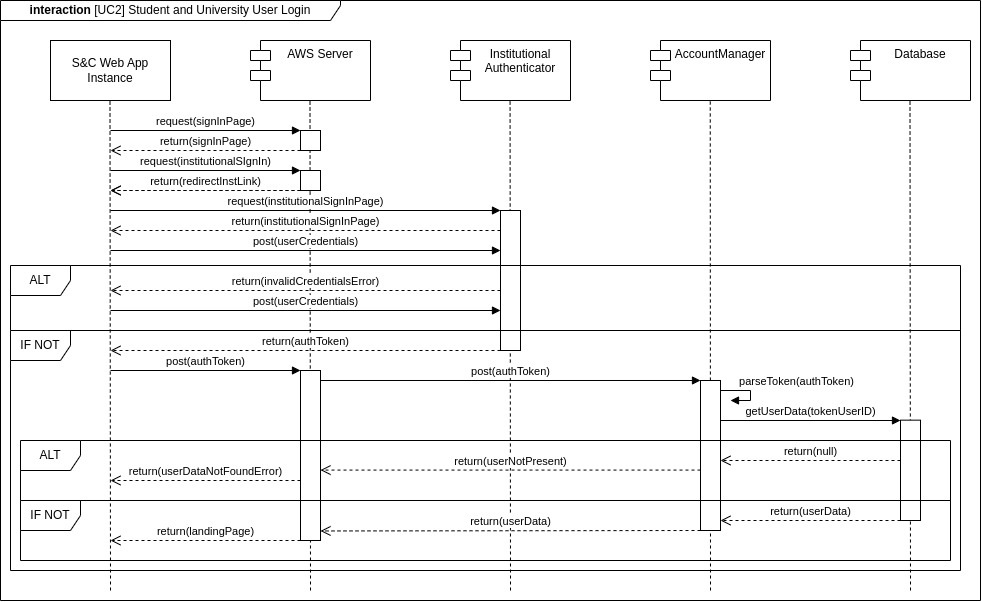
\includegraphics[width=1\linewidth]{DD-Latex//assets//Runtime View Diagrams/UC2.jpg}
        \caption{UC2 - Student and University User Registration}
        \label{fig:UC2}
    \end{figure}

    The second diagram can be considered a derivative of the first, as the communication process closely resembles that of the registration process. It should be noted that the final alternative flow depicted in this diagram actually marks the beginning of the registration process. If a user attempts to authenticate with an account that is not registered with the service, the system will automatically initiate the sign-in process.
    \newpage
    
    \item Register Company User
    \begin{figure}[h]
        \centering
        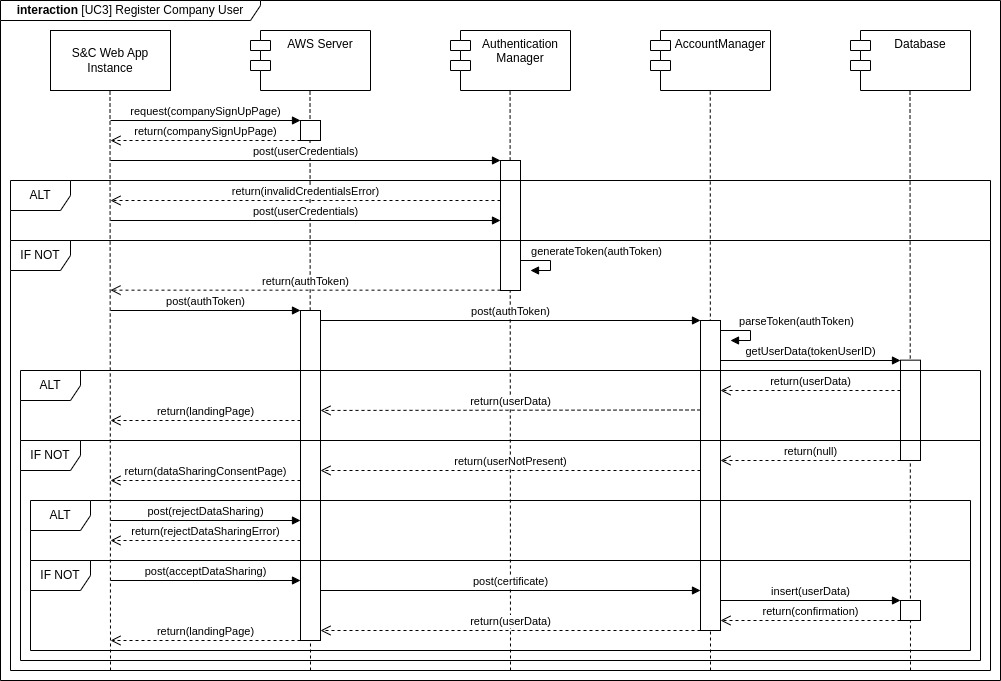
\includegraphics[width=1\linewidth]{DD-Latex//assets//Runtime View Diagrams/UC3.jpg}
        \caption{UC3 - Register Company User}
        \label{fig:UC3}
    \end{figure}
    
    The company user registration process is very similar to the student and university user registration, except that companies do not have access to external authentication services, unlike students and universities. The communication process remains largely the same throughout.

    \newpage
    \item Login Company User
    \begin{figure}[h]
        \centering
        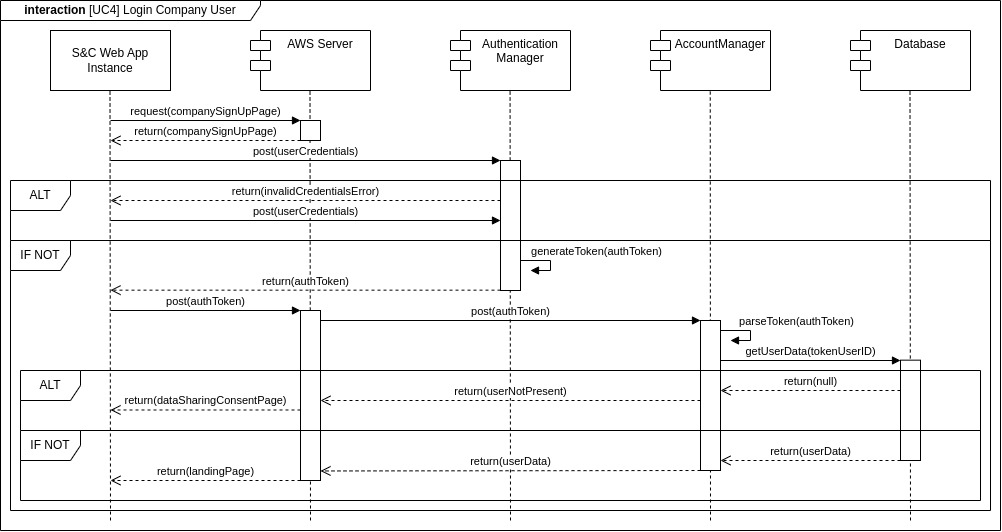
\includegraphics[width=1\linewidth]{DD-Latex//assets//Runtime View Diagrams/UC4.jpg}
        \caption{UC4 - Login Company User}
        \label{fig:UC4}
    \end{figure}
    
    As before, the login diagram is essentially a variation of the sign-up diagram, as the communication remains largely similar between the two processes. It should be noted that the final alternative flow presented leads to the option of signing up a new company user.
    
    \item Edit profile
    \begin{figure}[h]
        \centering
        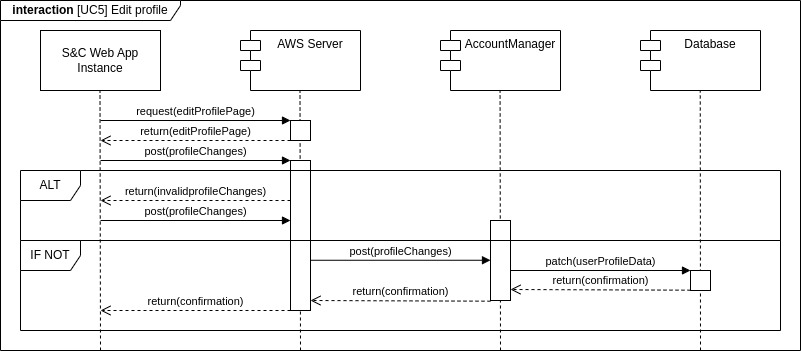
\includegraphics[width=1\linewidth]{DD-Latex//assets//Runtime View Diagrams/UC5.jpg}
        \caption{UC5 - Edit profile}
        \label{fig:UC5}
    \end{figure}

    The edit profile interaction assumes that the user is fully authenticated and has accessed the platform's landing page, as outlined in the original use case in the provided RASD v1 document. This explains the absence of the Authentication Manager component. Furthermore, the Account Manager component handles most of the required edits during this interaction.
    
    \item Create and Publish Internship Advertisement
    \begin{figure}[h]
        \centering
        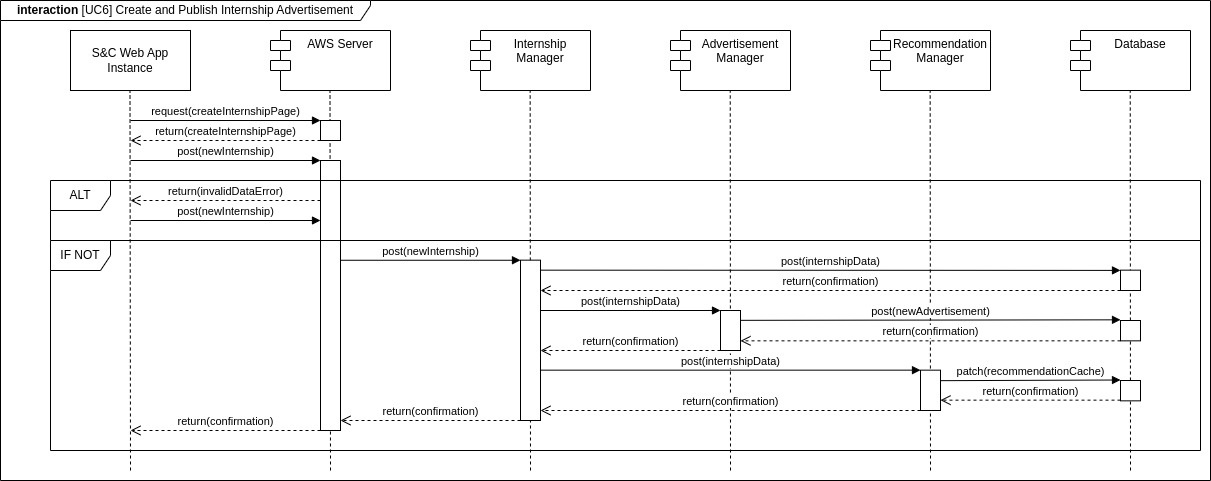
\includegraphics[width=1\linewidth]{DD-Latex//assets//Runtime View Diagrams/UC6.jpg}
        \caption{UC6 - Create and Publish Internship Advertisement}
        \label{fig:UC6}
    \end{figure}

    The sixth use case, which involves creating and publishing a new internship advertisement, includes some complex interactions to achieve the desired functionality. These interactions primarily occur between the Internship Manager, the Advertisement Manager, and the Recommendation Manager, as the latter two depend on the Internship Manager's functionality. The Internship Manager creates the internship in the database and then passes the relevant internship data to enable the creation and publication of the advertisement, as well as to update the recommendations cache.
    
    \item Edit Internship Advertisement
    \begin{figure}[h]
        \centering
        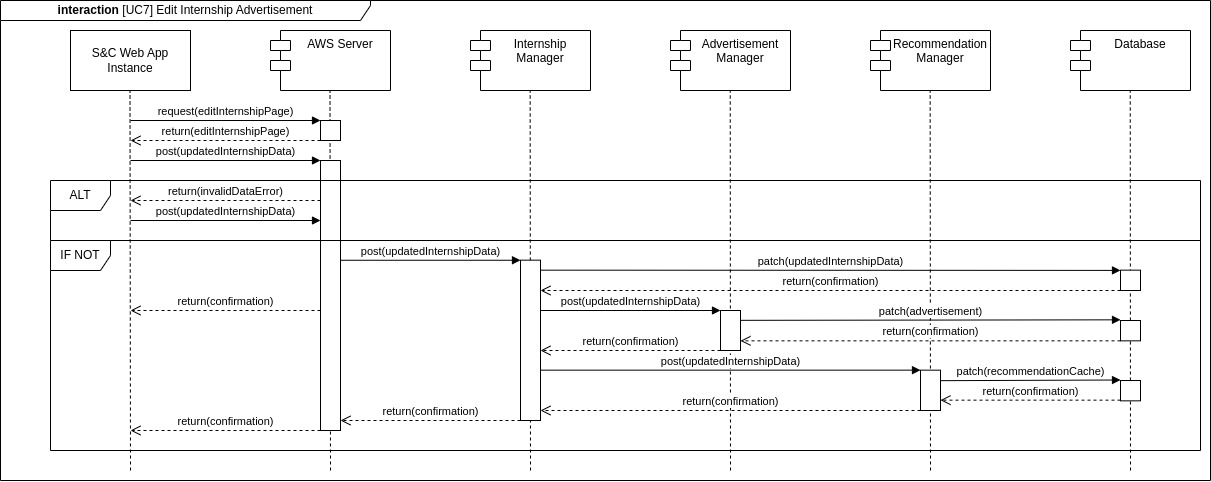
\includegraphics[width=1\linewidth]{DD-Latex//assets//Runtime View Diagrams/UC7.jpg}
        \caption{UC7 - Edit Internship Advertisement}
        \label{fig:UC7}
    \end{figure}

    The interactions required for editing an active internship advertisement are largely similar, if not identical, to those in UC6, with the main difference being the type of operations conducted between certain components (primarily, inserts being replaced with patches).
    
    \item Delete Internship Advertisement
     \begin{figure}[h]
        \centering
        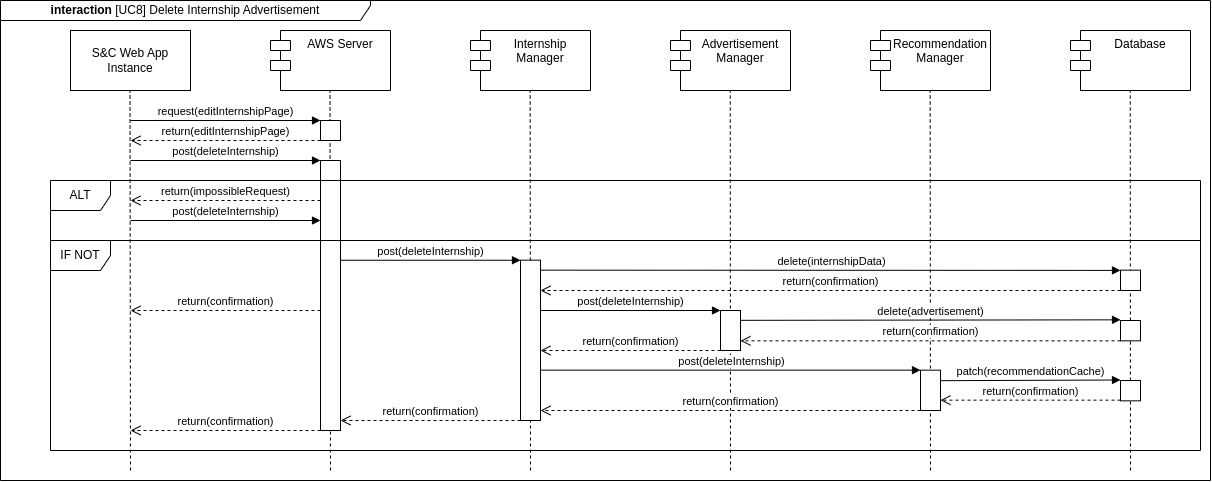
\includegraphics[width=1\linewidth]{DD-Latex//assets//Runtime View Diagrams/UC8.jpg}
        \caption{UC8 - Delete Internship Advertisement}
        \label{fig:UC8}
    \end{figure}

    As with the previous two use cases, the interactions between the components remain largely the same, with minor changes to the types of operations (specifically, inserts/patches being replaced by delete operations).
    
    \item View Recommendations \& Offerings, Apply for Internship
    \begin{figure}[h]
        \centering
        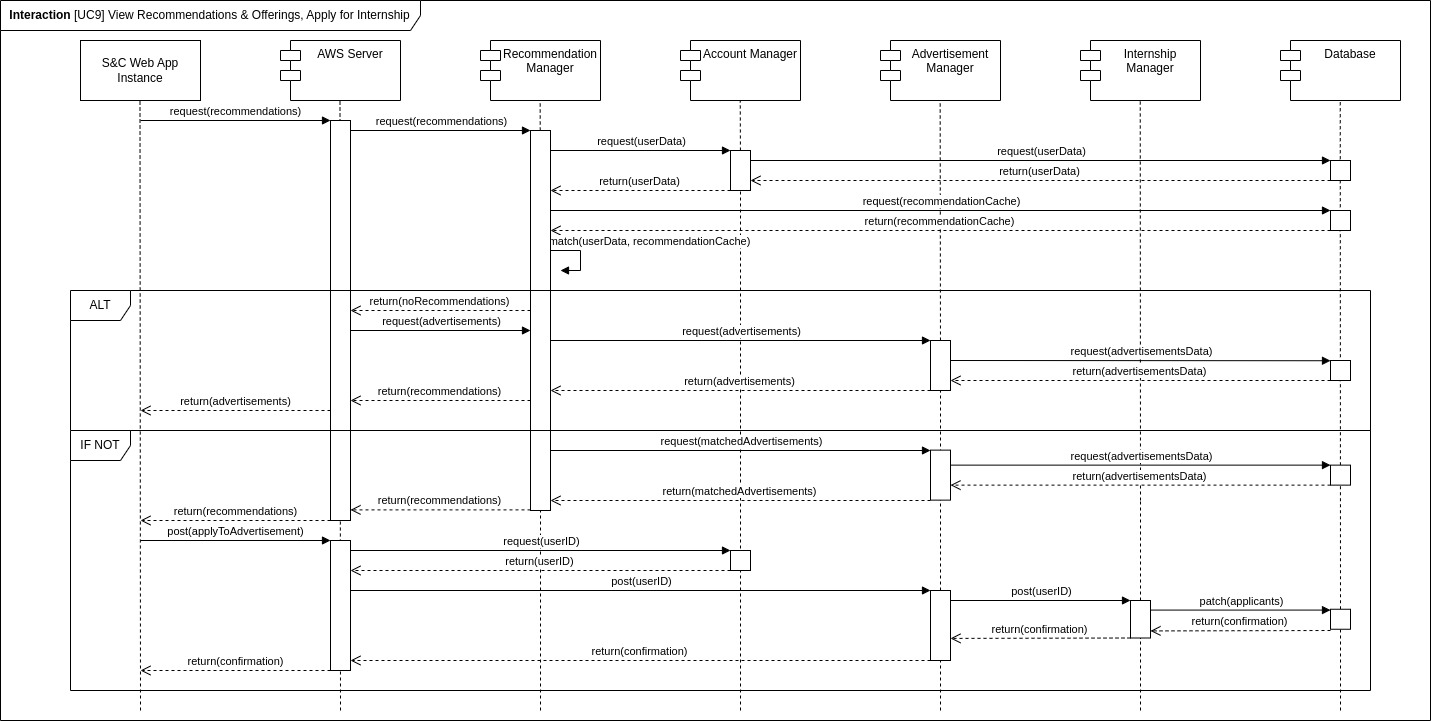
\includegraphics[width=1\linewidth]{DD-Latex//assets//Runtime View Diagrams/UC9.jpg}
        \caption{UC9 - View Recommendations \& Offerings, Apply for Internship}
        \label{fig:UC9}
    \end{figure}

    The UC9 Runtime View diagram represents one of the more complex diagrams in this section. For simplification, it can be divided into two stages: the first stage involves fetching or generating relevant recommendations for a single user, while the second stage covers the application process for a single internship advertisement.

    In the first stage, the Recommendations Manager gathers data based on the logged-in user's profile and retrieves its stored cache of internship advertisements from the database. Once the required data is retrieved, a matching algorithm runs to provide the user with advertisements relevant to their profile. An alternative flow exists where, if no match is found, the system returns a randomized set of advertisements.

    The second stage handles the application process, which involves much simpler inter-component communication compared to the first stage, as shown in the diagram.
    
    \item Change candidate status (increment or reject)
    \begin{figure}[h]
        \centering
        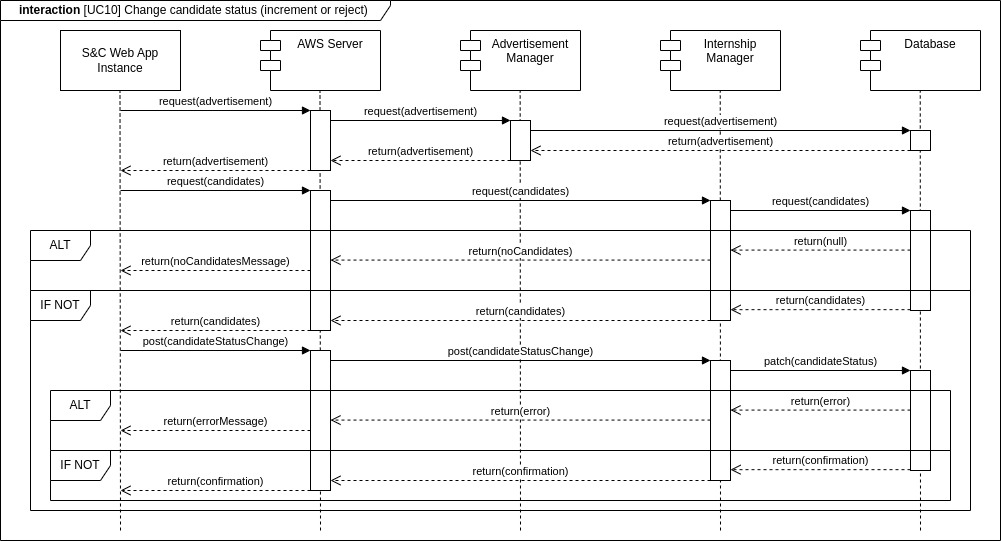
\includegraphics[width=1\linewidth]{DD-Latex//assets//Runtime View Diagrams/UC10.jpg}
        \caption{UC10 - Change candidate status (increment or reject)}
        \label{fig:UC10}
    \end{figure}

    UC10 illustrates the communication required to change a candidate's status. It begins by fetching all advertisements relevant to the user, and once one is selected, it retrieves all the candidates for that internship. An alternative flow exists for the scenario where no candidates have applied for the specific internship. Otherwise, the sequence continues by issuing a patch to the database for the selected candidate.

    \newpage
    \item Send Prompt to Candidate (questionnaire or interview invitation)

     \begin{figure}[h]
        \centering
        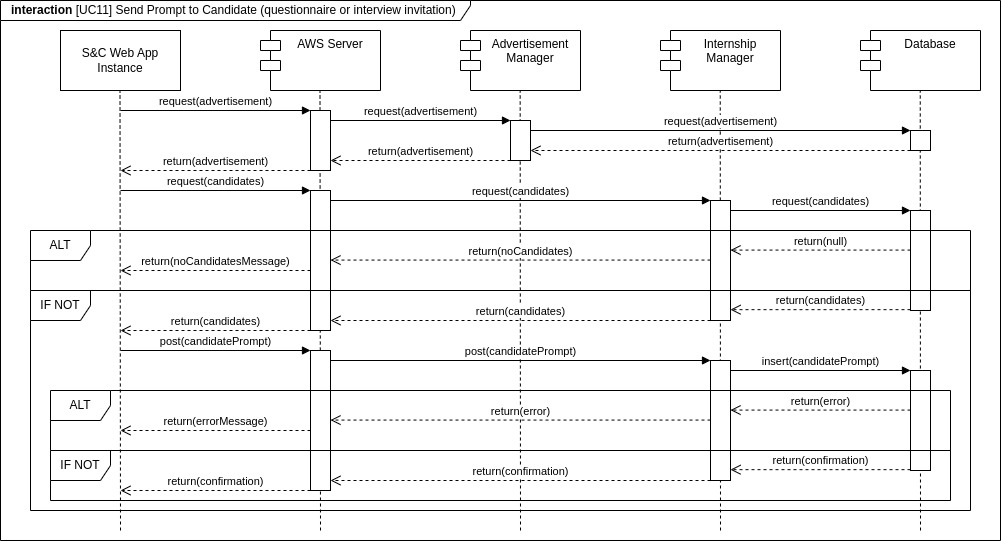
\includegraphics[width=1\linewidth]{DD-Latex//assets//Runtime View Diagrams/UC11.jpg}
        \caption{UC11 - Send Prompt to Candidate (questionnaire or interview invitation)}
        \label{fig:UC11}
    \end{figure}

    UC11 follows many of the same sequences presented in UC10, with the main differences lying in the types of communications between the components, such as patches being substituted for inserts.

    \item Reply to invitation

    \begin{figure}[h]
        \centering
        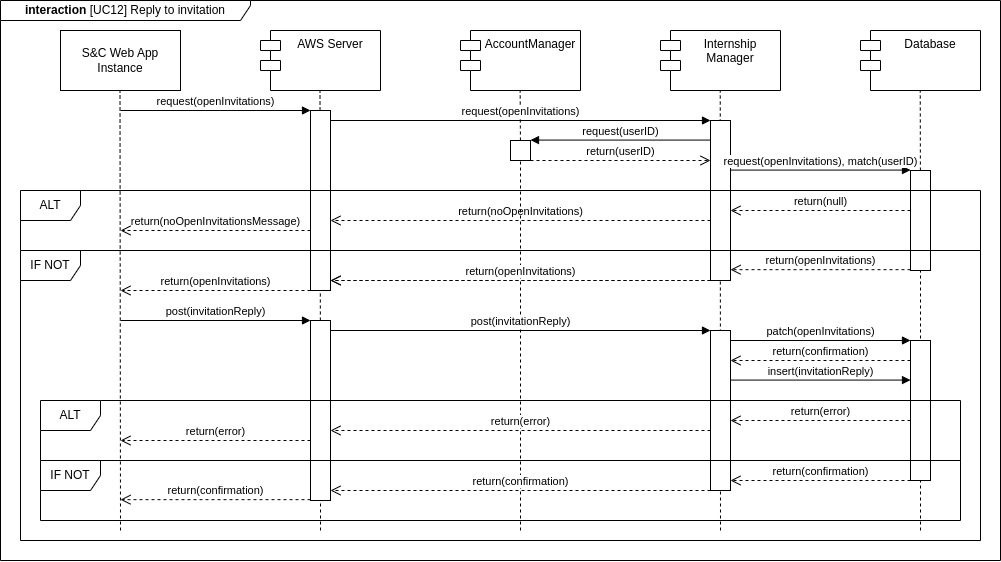
\includegraphics[width=0.90\linewidth]{DD-Latex//assets//Runtime View Diagrams/UC12.jpg}
        \caption{UC12 - Reply to invitation}
        \label{fig:UC12}
    \end{figure}

    Like UC11, the required interaction for UC12 is largely similar, but it contains a subtle difference, as two distinct database edits are required to complete it. First, a patch operation is performed to close the open invitation, followed by an insert operation to add the reply to the database.
    
    \item Initiate Internship
    \begin{figure}[h]
        \centering
        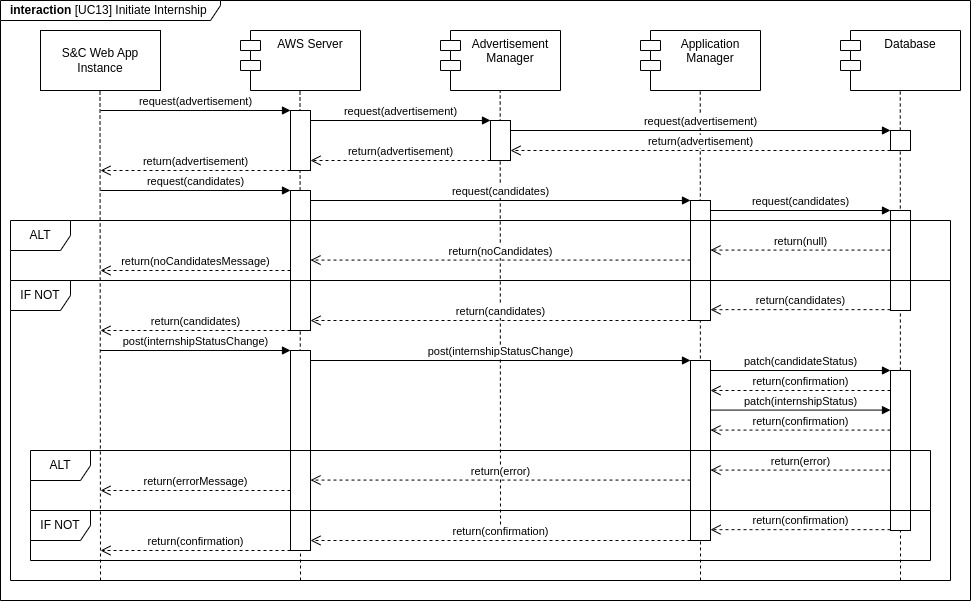
\includegraphics[width=1\linewidth]{DD-Latex//assets//Runtime View Diagrams/UC13.jpg}
        \caption{UC13 - Initiate Internship}
        \label{fig:UC13}
    \end{figure}

    UC13's communication process can be viewed as a mix of several presented use cases, with a degree of overlap between them. Ultimately, it comes down to having candidates who are eligible for the start of an internship, as well as two database edits required to initiate it.
    
    \item Submit Complaint

    \begin{figure}[h]
        \centering
        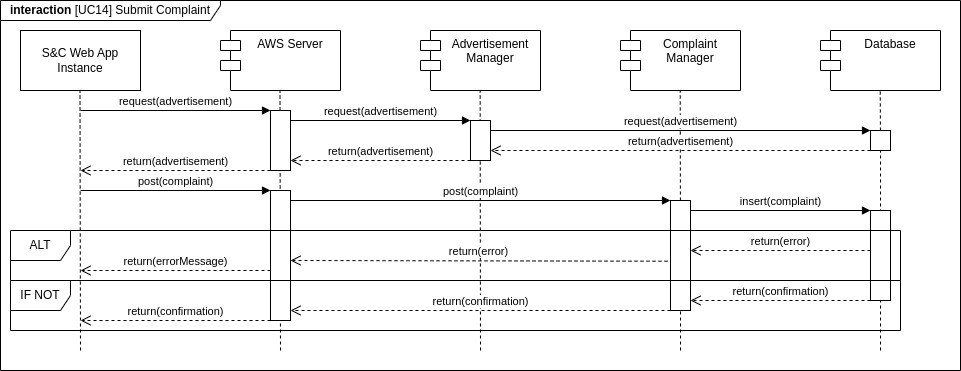
\includegraphics[width=1\linewidth]{DD-Latex//assets//Runtime View Diagrams/UC14.jpg}
        \caption{UC14 - Submit Complaint}
        \label{fig:UC14}
    \end{figure}

    The submit complaint runtime view is one of the simpler views in this document, as the interactions required among the components for its functionality are minimal. As shown in the diagram, the main actor is the complaint manager, who processes the complaint.
    
    \item Resolve complaint

    \begin{figure}[h]
        \centering
        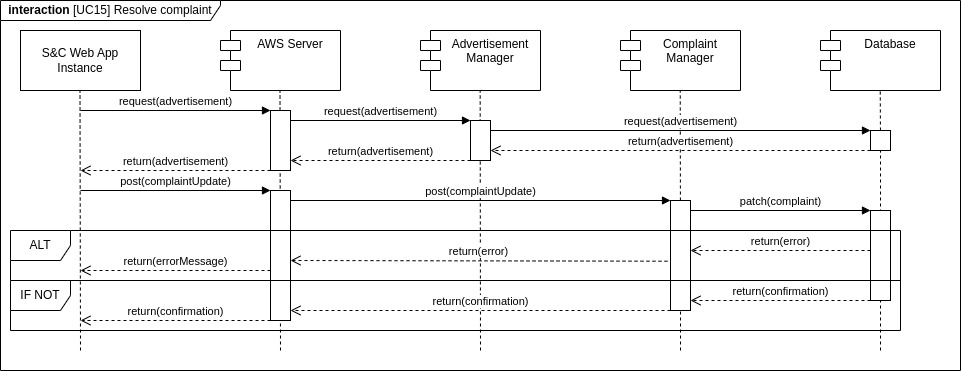
\includegraphics[width=1\linewidth]{DD-Latex//assets//Runtime View Diagrams/UC15.jpg}
        \caption{UC15 - Resolve complaint}
        \label{fig:UC15}
    \end{figure}

    As with many other use cases, UC15 is a simple variation of UC14, where the required operations are merely adjusted for the specific use case.
    
    \item Submit feedback

    \begin{figure}[h]
        \centering
        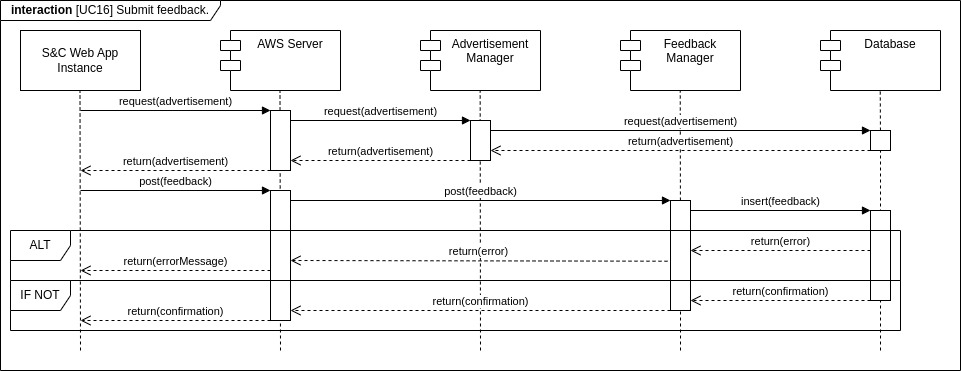
\includegraphics[width=1\linewidth]{DD-Latex//assets//Runtime View Diagrams/UC16.jpg}
        \caption{UC16 - Submit feedback}
        \label{fig:UC16}
    \end{figure}

    For the submission of feedback, there is a requirement that an internship be finished (either by its natural course or by early termination). Afterward, users may submit feedback, which is handled through the feedback manager, as shown in the diagram.
    \newpage
    
    \item View feedback

    \begin{figure}[h]
        \centering
        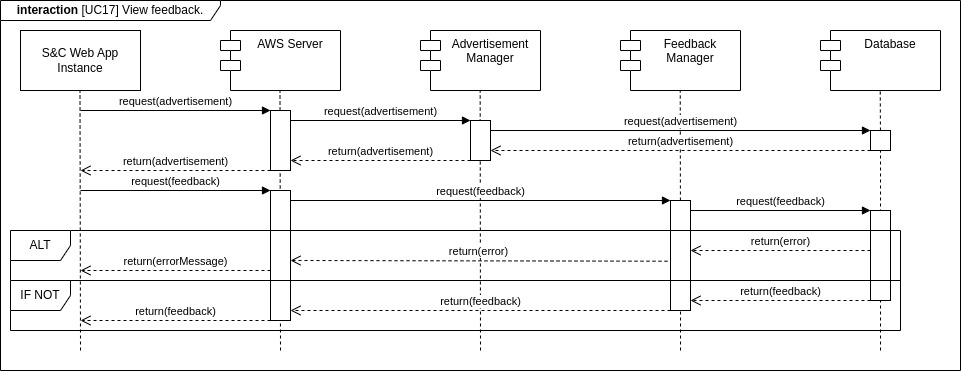
\includegraphics[width=1\linewidth]{DD-Latex//assets//Runtime View Diagrams/UC17.jpg}
        \caption{UC17 - View feedback}
        \label{fig:UC17}
    \end{figure}

    Lastly, the view feedback interaction is a simple variation of UC16, and like many of the previous ones, consists of minor changes in the types of interactions between the components.
\end{enumerate}